\chapter{Introduction}
\section{Preamble}
The race to autonomous driving is currently one of the main forces for pushing research forward in the automotive domain.
With highly automated vehicle prototypes gradually making their way to our public roads and fully-automated driving on the horizon, it seems to be a matter of time until we see robot taxis or cars navigating us through urban traffic or heavy stop-and-go on highways.
One major reason for this development in recent years is the rapid progress of \ac{AI}, especially the success of deep learning, which %drastically outperformed previous approaches 
has shown remarkable results in tasks essential for autonomous driving like object detection, classification \cite{Ciresan2012} and control \cite{Bojarski2016}.
Although more and larger data sets \cite{Geiger2013IJRR, Cordts2016} become available and powerful, parallelized computing hardware like \acp{GPU} facilitates training of increasingly deep network architectures \cite{Simonyan2014}, power consumption remains a critical issue. 
Especially in the automotive domain, energy-efficieny is of crucial importance.
Furthermore, current automated vehicle prototypes rely on a vast diversity of redundant sensory systems to perceive sufficient information about the outside world \cite{Aeberhard2015}.
In contrast, human drivers are capable of handling challenging driving situations under changing environmental conditions by using mainly the human eyes as primary sensor input and the brain for information processing.
Furthermore, the human brain is also comparably small and efficient consuming only \SI{20}{\watt} of power (equivalent to a compact fluorescent light bulb) while comprising \SI{2}{\percent} of the body weight \cite[Chap. 2.1]{Eliasmith2013}.
Therefore, the focus of the young and emerging research field neuromorphic engineering is on biologically inspired computing systems and algorithms, aiming to close the gap in performance and efficiency between biological and artificial computing systems.
Although the neuromorphic prototypes of computing hardware, e.g. \ac{SpiNNaker} \cite{Furber2014} or  IBM's TrueNorth \cite{Akopyan2015}, dedicated to processing so-called \acp{SNN} are not technologically mature yet, they show promise to be a useful addition in future automotive applications.
Since these novel spiking-neuron architectures encapsulate a drastically different computing paradigm compared to the conventional von-Neumann architecture \cite{vonNeumann1993}, they also call for alternative algorithmic approaches and new programming substrates (e.g. \cite{Amir2013}).\\
In this thesis, we investigate potential applications of neuromorphic approaches in automotive context.
Given the complexity of driving a car autonomously in all possible real-world situations, tackling the complete set of all necessary tasks is out of scope of a single thesis.
Therefore, we need to focus on certain sub-tasks.
Regarding this selection process, we contemplate two concepts.
We categorize tasks necessary for highly automated driving using the perception-action-cycle and rate their level of complexity using Moravec's paradox \cite{Moravec1988}.
Moracev's paradox postulates the observation, that tasks or skills that seem effortless to humans are harder to reverse-engineer than tasks we experience or expect to be difficult.
Moracev argues, that we learned those seemingly effortless skills over billions of years of evolution through experience about the nature of the world such that they became unconscious to us.
A good example of this paradox is the fact that artificial systems are already able to defeat the world's best human players in games like Chess \cite{Hsu2002} or Go \cite{Silver2016}, which are considered particularly difficult by humans.
On the other hand, we are still struggling to create robots that solve seemingly effortless sensorimotor tasks like climbing stairs or opening doors \cite{Guizzo2015, Norton2017}.\\
The perception-action-cycle \cite{Fuster2004} is the concept of a circular information flow between an organism or agent (living or artificial) when interacting with its environment through goal-directed behaviour (cf. Fig. \ref{fig:perc-act-cicle}). 
\begin{figure}[t!]
	\centering
	%	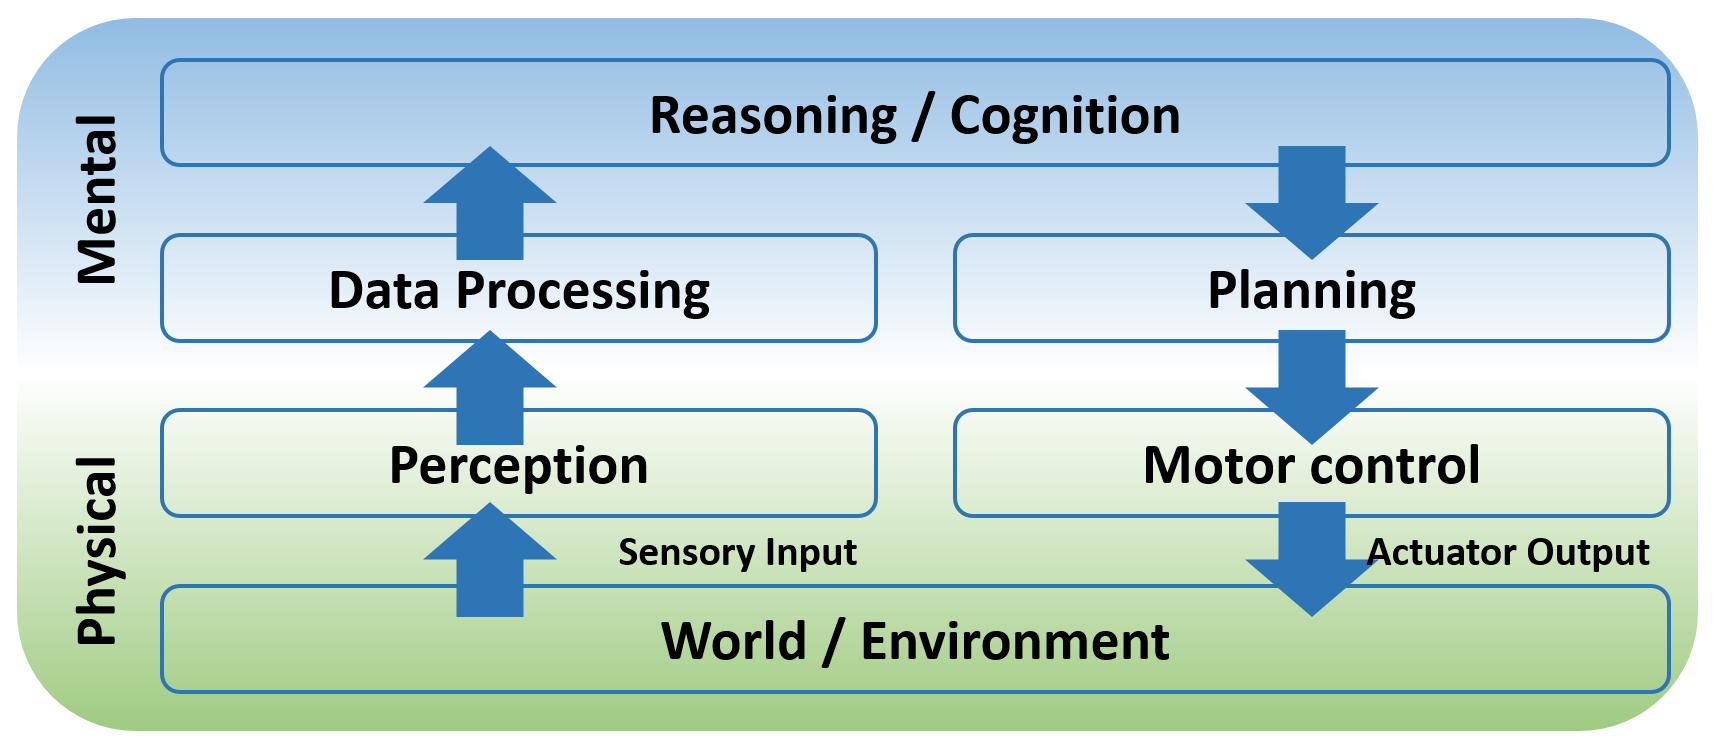
\includegraphics[width=0.85\textwidth, height=150px]{imgs/ActionPerceptionCycle.eps}
	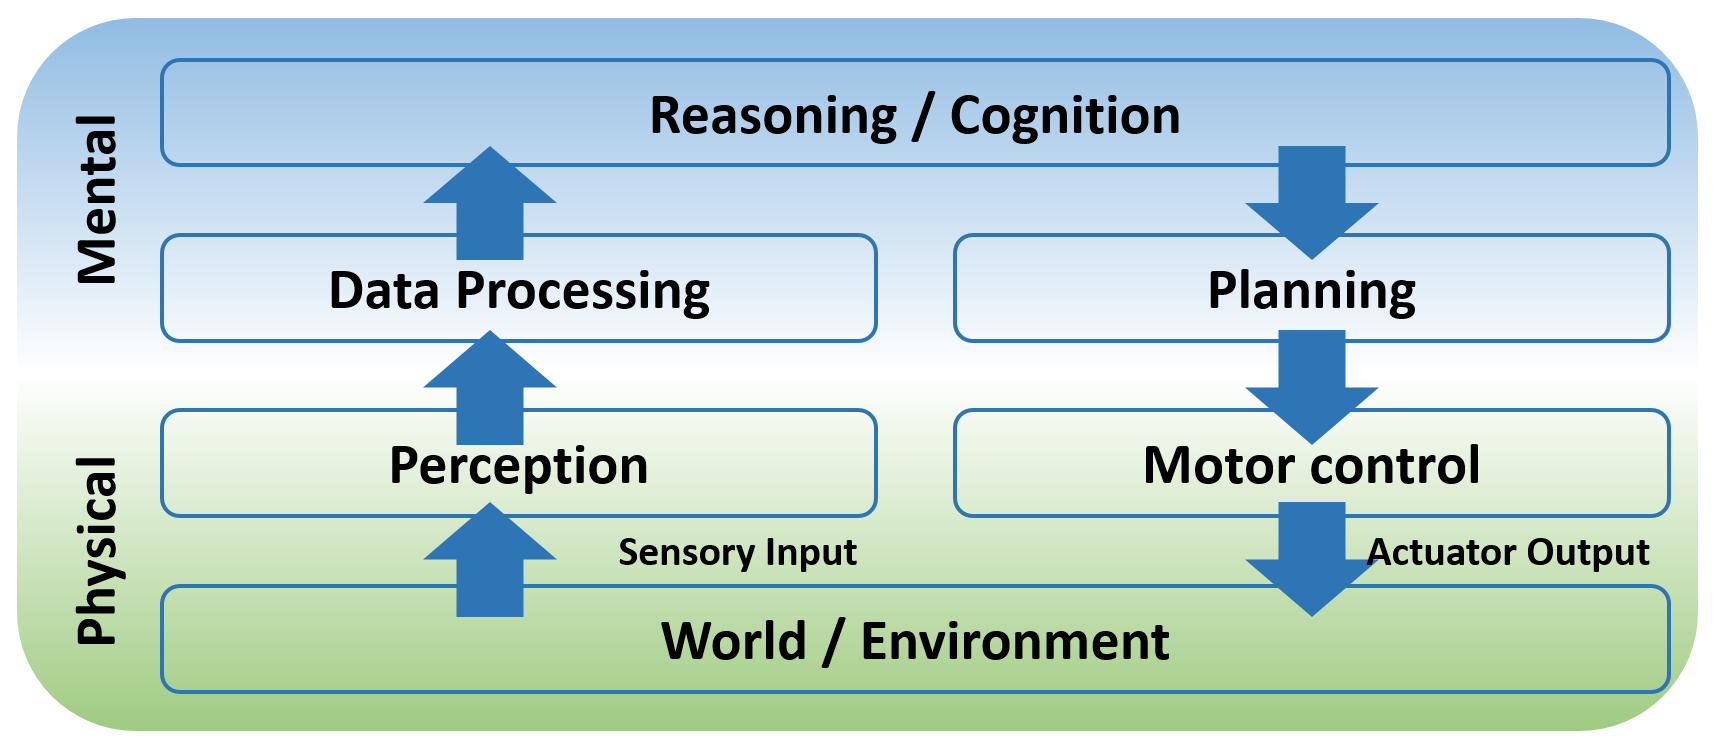
\includegraphics[width=0.85\textwidth]{imgs/ActionPerceptionCycle.eps}
	\caption{Schematic visualization of the perception-action-cycle}
	\label{fig:perc-act-cicle}
\end{figure}
Instead of considering the directional aspects of the cycle in the opposite categories of perception and action, it is also common to separate tasks in terms of hierarchy \cite{Loeb2014}.
Interaction with the physical world through sensing and manipulation is considered on lower hierarchical level within the perception-action-cycle while formation of mental representations and reasoning about them reside on a higher level. 
We refer to those different hierarchical levels as \emph{physical} and \emph{mental} or \emph{lower} and \emph{upper} interchangeably.\\
Considering the physical/lower level of the perception-action-cycle, \acp{DNN} have recently shown significant progress and success at perception tasks like object detection and classification.
Therefore, we believe a lot more research is necessary until neuromorphic approaches using \acp{SNN} are sufficiently mature to compete with those traditional approaches, although current work in this directions shows promising results \cite{Hunsberger2015}.
Similar arguments hold true for automated learning approaches regarding vehicle control.
Although sophisticated learning techniques show promise to improve motor control, to date most controllers for automated vehicles or robots in general "designed and tuned by human engineers" \cite{Deisenroth2013}.
One of the main reasons is the fact that control of an automated vehicle is an extremely safety-critical domain, while at the same machine learning approaches in general pose additional challenges regarding safety validation \cite{Koopman2016}.
Furthermore, those tasks on the physical level of the perception-action-cycle are solved effortlessly by humans and therefore, according to Moravec's paradox, we should expect them to be hard to master for artificial learning systems.\\
Therefore, we decided to focus on the mental/upper part of the perception-action-cycle in this thesis.
On the one hand, we believe that tasks in this part of the cycle show promise to benefit most from neuromorphic approaches. 
On the other hand, "mental" tasks do not necessarily need to be performed and evaluated in closed-loop systems, which make them less problematic regarding safety issues, and therefore ideal candidates for further investigations.\\
Precise knowledge about the current environment state and its future development is essential for an autonomous agent to plan a secure path for navigation and to safely interact with the world. 
In case of highly automated vehicles, perception of the outside world usually happens through a variety of different sensory systems like cameras, \acs{RADAR} and \acs{LIDAR} sensors \cite{Aeberhard2015}. 
This observed information needs to be collected and combined into a central environment model, which is the (mental) basis for further reasoning and decisions.
One essential ingredient for such a model of the environment, or mental tasks in general, is knowledge or information representation.
It is an open research question to date, how the human brain represents knowledge and what underlying neural or computational substrate it uses to encode information \cite{Wang2003, Samsonovich2012, Handjaras2016}.
Most modern approaches to reasoning or cognitive tasks in context of robotics or automated driving are built upon Bayesian probability theory and use "computer-scienetific" approaches to knowledge representation.
This could be lists of objects (cf. Fig. \ref{subfig:urban_object_lists}) with numerical encoding of properties when working on a higher level of abstraction.
On a lower level, another common approach especially in context of neural-network learning, is to label raw sensory data, for example individual pixels of images (cf. Fig. \ref{subfig:urban_semantic_labels}).
However, when we as humans observe a particular scene (e.g. while driving), our mental representation will probably be very different from those aforementioned approaches.
\begin{figure}[t!]
	\centering
	\subfloat[Urban traffic scenario\label{subfig:urban_scene}]{%
		\includegraphics[width=0.45\textwidth]{imgs/urban_scene.eps}
	}
	\subfloat[Pixel-wise labels\label{subfig:urban_semantic_labels}]{%
		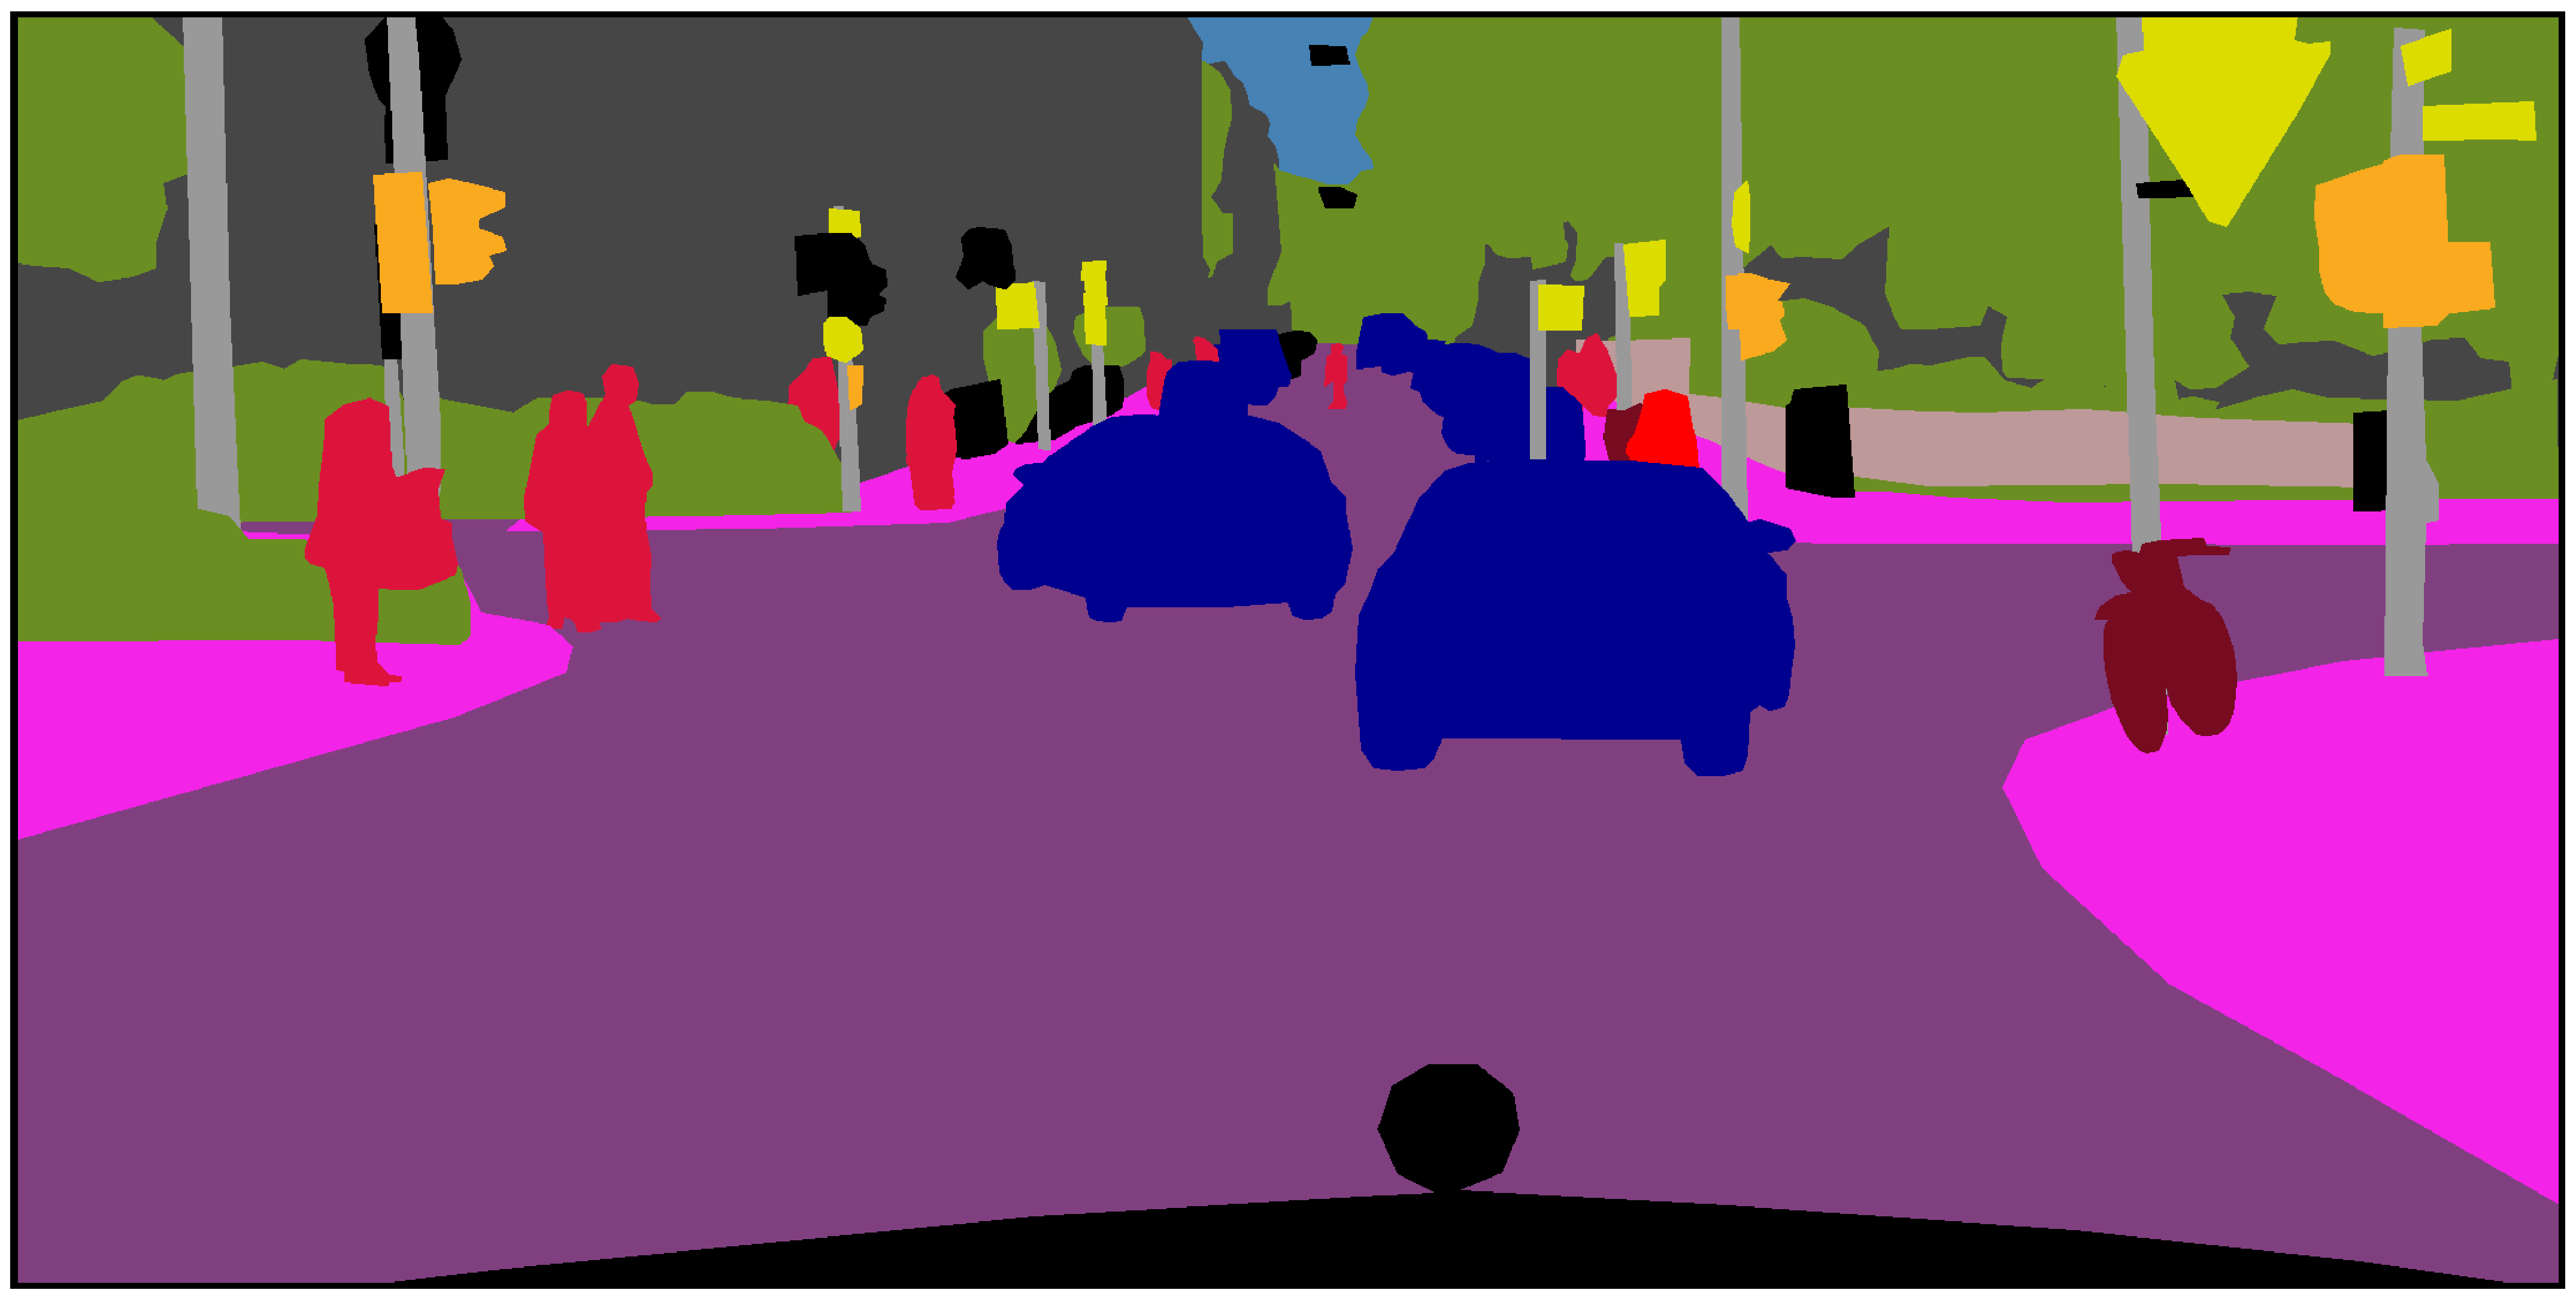
\includegraphics[width=0.45\textwidth]{imgs/urban_scene_pixel_labels.eps}
	}\\
	\subfloat[Bounding boxes indicating objects of interest\label{subfig:urban_scene_boxes}]{%
		\includegraphics[width=0.45\textwidth]{imgs/urban_scene_bound_boxes.eps}
	}
	\subfloat[Exemplary representation using lists of objects\label{subfig:urban_object_lists}]{%
		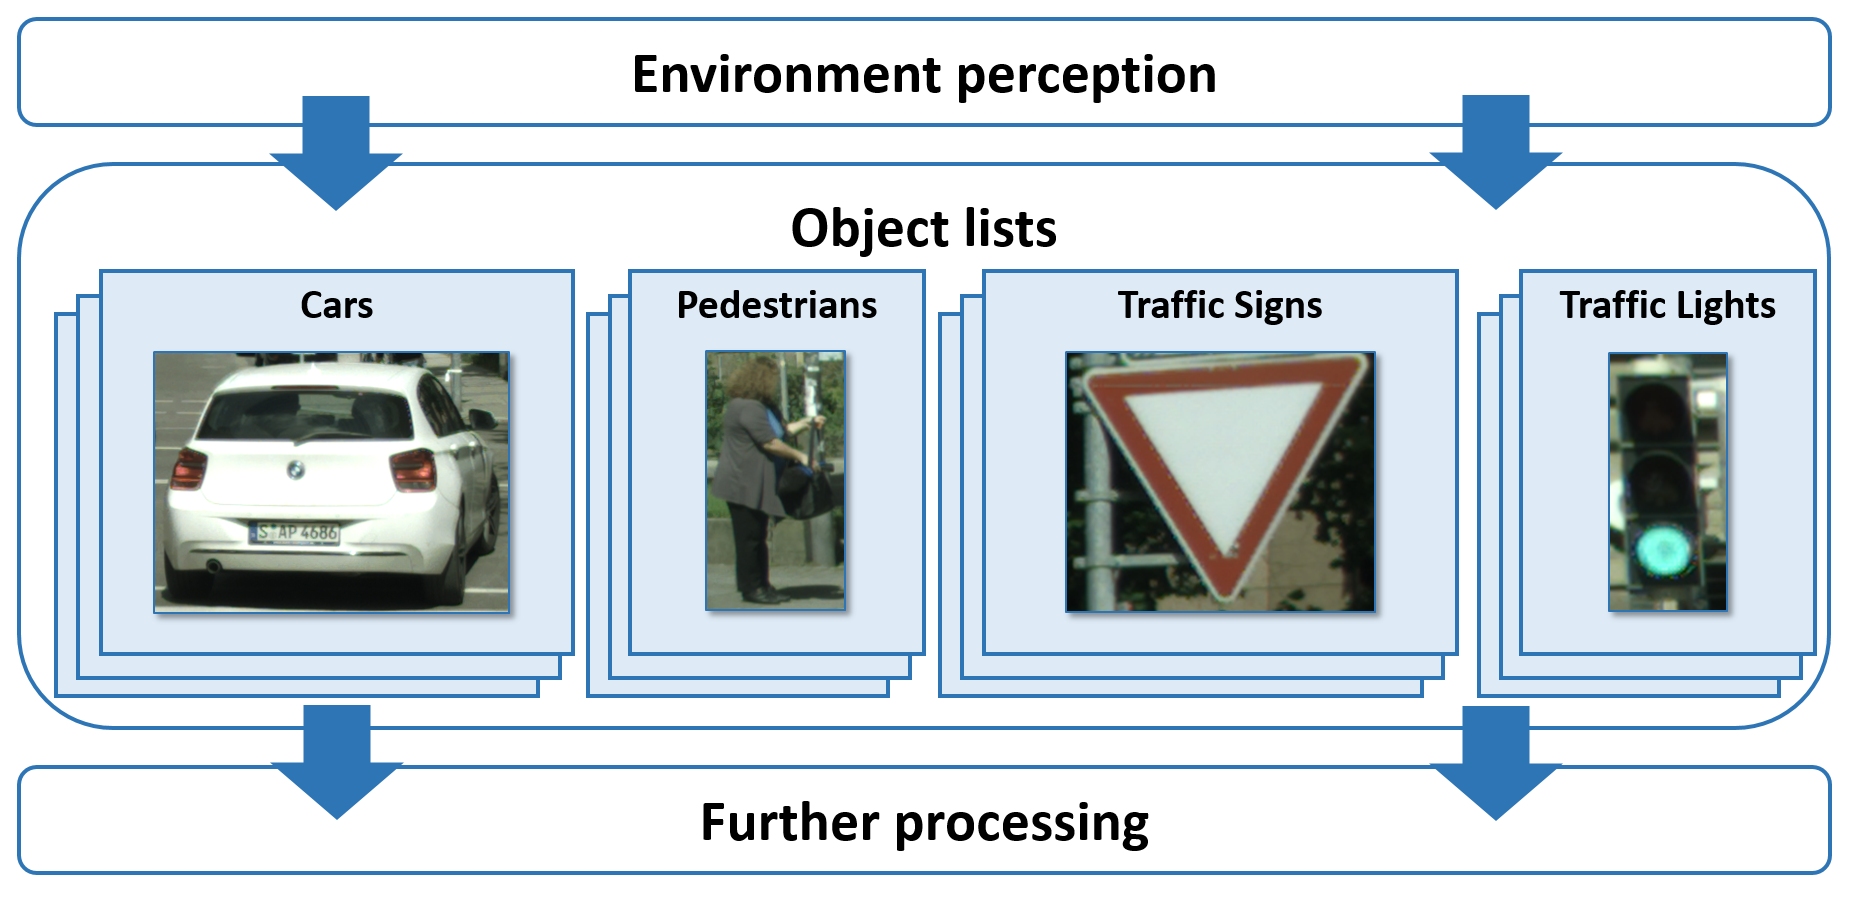
\includegraphics[width=0.45\textwidth, height=3.6cm]{imgs/urban_scene_object_lists.eps}
	}
	\caption{Example of urban driving scene with different approaches to representation. Images \ref{subfig:urban_scene}, \ref{subfig:urban_semantic_labels} and \ref{subfig:urban_scene_boxes} are (adapted) from the Cityscapes-dataset \cite{Cordts2016}}\label{fig:urban_scene}
\end{figure}
A human observer's representation/description of Fig. \ref{subfig:urban_scene} would probably be in a semantic/linguistic form, like \emph{a blue car turning left, a white car turning right, three pedestrians waiting on the left side of the road, green traffic lights, a yield way sign} etc.
One common approach to encode such conceptual, semantic information or, more generally, natural language in computer-readable fashion is by using vector representations.
\acfp{VSA} is a term coined by Ross W. Gayler \cite{Gayler2003} to cover this family of modelling approaches that represent symbols or structures by mapping them to (high-dimensional) vectors.\\
In this thesis, we investigate the use of these vector representations for knowledge representation and reasoning in context of automotive environment modelling.
This approach to information encoding is rather generic and can be applied to various different tasks with little modifications to the representation itself. 
Furthermore, \acp{VSA} are suitable as inputs to \acp{SNN} \cite{Eliasmith2013}, which support efficient learning algorithms and deployment on dedicated neuromorphic hardware. 
This allows us to combine the advantages of symbolization with the benefits of neural networks.
We investigate varying instantiations of our representation applied to different applications. \todo{see if we still need this phrase of if we focus more or less completely on behaviour prediction}
One essential ingredient of an environment model especially in automotive context is precise knowledge about the current state and future development of all dynamic objects in the ego-vehicle's surroundings.
We focus on the task of predicting the behaviour of those other traffic participants around the ego-vehicle based on a vector description of the current scene.
These structured representation have the potential to capture mutual interactions between dynamically moving agents.
Prediction of other traffic participants behaviour also offers the opportunity to explore different learning approaches.
Human drivers have acquired comprehension through past experience of how other cars will probably act, but adapt this knowledge continuously when encountering new situations.
From this inspiration, we aim to learn a generic model of dynamic behaviour through offline (i.e.batch) training and refine this model when perceiving behaviour of a particular object through online learning.
One major challenge here is to ensure that online learning will adapt and improve overall performance without losing the knowledge acquired through batch training.

\section{Outline of the thesis}
This section provides a brief overview of the thesis structure as well as a short summary for each chapter.